\section{Anforderungen}
Um sicherstllen zu k\"{o}nnen, dass das Projektziel bestm\"{o}glicht erreicht wird, wurde eine Anforderungsliste erstellt, mit deren Hilfe die G\"{u}te der Umsetzung des Versuchskonzepts gemessen werden kann. Diese Liste enth\"{a}lt die Anforderungen des Auftraggebers und unseren eigenen, welche sich aus den zu Grunde liegenden technischen Dokumenationen der verwendeten Messger\"{a}te und den VDI Richtlinien f\"{u}r Reinraumtechnik ergeben haben.\\
Bei den festgelegten Anforderungen war uns eine genaue Quantifizierung der Werte wichtig, wann immer es m\"{o}glich war. Bei den Anforderungen wird zwischen den folgenden Arten unterschieden:

\begin{enumerate}
	\item \textbf{Festforderung} (FF): Es muss ein bestimmter Wert aufweisbar sein und Abweichungen davon sind nicht zul\"{a}ssig.
	
	\item \textbf{Bereichsforderung} (BF): Die Anforderung muss einen Wert aufweisen und dieser darf nur innerhalb eines bestimmten Bereich liegen.
	
	\item \textbf{Mindestforderung} (MF): Bei einer Mindestforderung muss die Anforderung mindestens einen angegeben Wert aufweisen.
	
	\item \textbf{Zielforderung} (ZF): Der Wert einer Anforderung muss bei einer ZF m\"{o}glichst nah an einem Zielwert liegen, um gut bewertet werden zu k\"{o}nnen.
	
	\item \textbf{Wunsch} (W): Da es sich um einen Wunsch handelt, ist die Wichtigkeit des Merkmals vergleichsweise gering. Die Anforderung sollte dann allerdings einen bestimmten Wert aufweisen und wird bei der Bewertung positiv ber\"{u}cksichtigt. 
\end{enumerate}
F\"{u}r die Generierung eines Partikeltestsignals in Form einer Sprungfunktion lassen sich die folgenden Anforderungen festlegen, die sich in drei Kategorien unterteilen lassen:
\begin{enumerate}
	\item \textbf{Aerosolquelle}: Anforderungen an die Quelle, welche das Pr\"{u}faerosol erzeugt
	\item \textbf{Aerosol}: Anforderungen an das Pr\"{u}faerosol, welches dem zu testenden Messger\"{a}t zugef\"{u}hrt wird
	\item \textbf{Schaltvorrichtung}: Anforderungen an die Schaltvorrichtung, welche den Partikelsprung erm\"{o}glicht 
	\item \textbf{Aerosolleitungen}: Anforderungen an die Schnittstelle, welche die Aerosolquelle mit dem Messger\"{a}t verbindet
	\item \textbf{Versuchsaufbau}: Anforderungen an den gesamten Versuchsaufbau inklusive der verwendeten Ger\"{a}te
\end{enumerate}
\begin{longtable}{| l | l | l | l | l | l |}
	\caption{Anforderungen mit anschlie{\ss}enden Erl\"{a}uterungen}\label{anforderungsliste}\\
	\hline
	
	\textbf{Anforderung} & \textbf{Nr.} & \textbf{Art} & \textbf{Wert} & \textbf{Einheit} & \textbf{Quelle}\\

	\hline

	Druck am  & 1 & BF & Eingang - Ausgang & $kPa$ & Datenbl\"{a}tter\\
	Messger\"{a}teeinlass& & & $70 - 103$ (FMPS) & &\\
	& & & $40 - 103$ (APS) & &\\
	& & & $<0.746$ (OPS) & &\\
	& & & $75-105$ (UCPC) & &\\
	
	\hline
	
	Einstellzeit der & 2 & ZF & 0 & $s$ &selbstgew"{a}hlte\\
	Partikelanzahlkonzentration & & & & &Last\\
	der Aerosolquelle & & & & &\\
	
	\hline
	Tr\"{a}gergas& 3 & FF & & & Datenbl\"{a}tter\\
	- gefilterte Luft & & & & &\\
	
	\hline
	
	Volumenstrom & 4 & FF & 10 (FMPS) & $l/min$ & Datenbl\"{a}tter\\
	(Tr\"{a}gergas) & & & $5 \pm 0.2$ (APS)& &\\
	& & & $1 \pm 0.05$ (OPS)& &\\
	& & & $1.5 \pm 0.05$ (UCPC)& &\\
	
	\hline
	
	Tr\"{a}gergastemperatur & 5 & BF & $283.15-325.15$(FMPS) & $K$ & Datenbl\"{a}tter\\
	& & & $283.15-313.15$(APS) & &\\
	& & & $273.15-318.15$(OPS) & &\\
	& & & $283.15-308.15$(UCPC) & &\\
	
	\hline
	
	Partikelanzahlkonzentration & 6 & BF & $100-10^{7}$ (FMPS)& $n/cm^{3}$ & Datenbl\"{a}tter\\
	& & & $0,001-1000$ (APS) & &\\
	& & & $0-3000$ (OPS) & &\\
	& & & $0-3\cdot10^{5}$ (UCPC) & &\\
	
	\hline
	
	Partikelmaterial (Messger\"{a}t) & 7 & W &  &  & Datenblatt APS\\
	- feste Schwebeteilchen & & & & &\\
	
	\hline
	
	Partikelgr\"{o}{\ss}e & 8 & BF & $5.6-560$ (FMPS) & $nm$ & Datenbl\"{a}tter\\
	& & & $500-20000$ (APS) & &\\
	& & & $300-10000$ (OPS) & &\\
	& & & $2.5-3000$ (UCPC) & &\\
	
	\hline	
		
	Schaltzeit & 9 & ZF & 0 & s & selbstgew\"{a}hlte\\
	& & & & & Last\\
	
	\hline
	
	Str\"{o}mungsbeg\"{u}nstigender & 10 & ZF & 0 & n & VDI 3491\\
	Schaltvorgang & & & & &\\
	
	\hline	
			
	Weg zwischen Umschaltvorrichtung & 11 & ZF & 0 & m & selbstgew\"{a}hlte\\ 
	und Messger\"{a}teinlass & & & & & Last\\
	
	\hline
	
	Laminarer Strom & 12 & MF & $< 2300$ & - & VDI 3491\\
	& & ZF & $1500$ & &\\
	
	\hline
	
	Schnittstelle zum & 13 & FF & 9.5 (FMPS) & $mm$ & Datenbl\"{a}tter\\
	Messger\"{a}t (Inlet) & & & 19 (APS) & &\\
	& & & 6.35 (OPS) & &\\
	& & & 6.4 (UCPC) & &\\
	
	\hline		
		
	Pr\"{u}fzeit & 14 & ZF & 3300 & $s$ & selbstgew\"{a}hlte\\
	& & & & & Last\\
	
	\hline
	
	Kosten & 15 & ZF & 0 & Euro & Vorgabe \\
	& & BF & $0-1000$ & &\\
	
	\hline
	
	Anzahl Messger\"{a}te& 16 & MF & $\geq2$ (FMPS, OPS) & $n$ & Vorgabe\\
	
	\hline
\end{longtable}

\subsection{Messger\"{a}te}
Bei der Konzeption der Versuchsaufbauten sollte anfangs darauf geachtet werden, dass mit diesen verschiedene Messger\"{a}te unterschiedlicher Hersteller getestet werden k\"{o}nnen. Im Verlauf des Projekts wurde zur Vereinfachung des Konzeptentwurfs nach Absprache mit dem Auftraggeber sich darauf geeinigt, sich auf die Messger\"{a}te \textbf{Fast Mobility Particle Sizer Spectrometer Model 3091} (kurz FMPS 3091) und \textbf{Optical Particle Sizer Model 3330} (kurz OPS 3330) der Firma \textbf{TSI} zu konzentrieren. 

Es bestand dennoch weiterhin die Schwierigkeit geeignete Anforderungen zu identifizieren, die die Versuchsaufbauten erf\"{u}llen m\"{u}ssen, um sie zumindest auf die Ger\"{a}te FMPS 3091 und OPS 3330 anwenden zu k\"{o}nnen. Die Gr\"{u}nde hierf\"{u}r liegen in ihren unterschiedlichen Leistungen und Funktionsrinzipien. Abbildung \ref{fig:verfahren} zeigt einen \"{U}berblick \"{u}ber die heutigen verf\"{u}gbaren Messverfahren. Die Wahl eines Verfahrens h\"{a}ngt unter anderem davon ab, welche Partikelgr\"{o}{\ss}en gemssen werden sollen. 

\begin{figure}[H]
	\myfloatalign
	{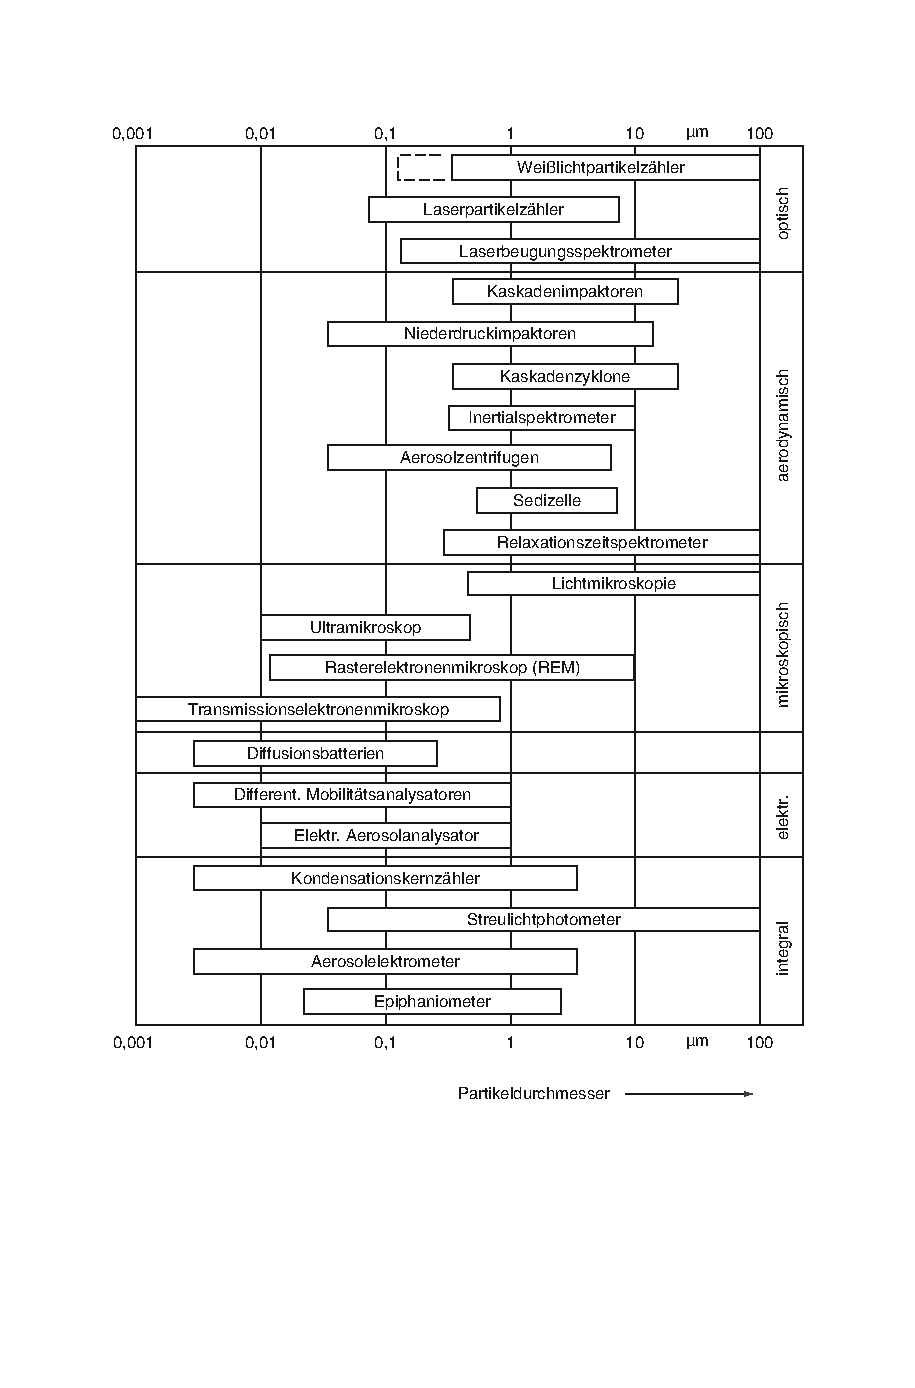
\includegraphics[width=.9\linewidth]{gfx/requirements/partikelmessverfahren.pdf}} \quad
	\caption[\"{U}bersicht \"{u}ber gebr\"{a}chliche Partikelmessverfahren (Quelle: \cite{reinraum}, S.71)]
	{\"{U}bersicht \"{u}ber gebr\"{a}chliche Partikelmessverfahren (Quelle: \cite{reinraum}, S.71)}
	\label{fig:verfahren}
\end{figure}

Optische Partikelz\"{a}hler arbeiten nach dem physikalischen Prinzip, dass beleuchtete Partikel das Licht aus seiner urspr\"{u}nglichen Ausbreitungsrichtung ablenken (Abbildung \ref{fig:optischer_messer}). Bei diesen passiert jeder einzelne Partikel ein Messvolumne, in dem er von Licht bestrahlt wird und dann mit Hilfe eines Detektors die Intensit\"{a}t des gestreuten Lichts und die Anzahl der gestreuten Lichtimpulse gemessen. Die Intensit\"{a}t l\"{a}sst Aufschl\"{u}sse \"{u}ber die Partikelgr\"{o}{\ss}e ziehen, bei einem bekannten Volumenstrom und vordefinierter Messdauer l\"{a}sst sich \"{u}ber die Anzahl der Lichtimpulse die Partikelkonzentration bestimmen. Bei moderneren Ger\"{a}ten wie dem OPS 3330 geschieht die optische Messung mit Hilfe eines Laser (Abbildung \ref{laser_messer}). Hierbei kommt zus\"{a}tzlich ein Parabolspiegel hinzu, mit dem das gestreute Licht von einem Detektor gesammelt wird. Bei diesem Messprinzip ist es wichtig, dass jeder Partikel das Messvolumen einzeln durchlaufen muss. Falls zwei oder mehr Partikel das Messvolumen gleichzeitig durchlaufen, werden sie als ein Gro{\ss}es gewertet. Dieser Effekt wird als Koinzidenz bezeichnet. Es existieren zwei Methoden, um diesen Effekt zu vermeiden. Die erste Methode arbeitet aerodynamisch, bei welcher der Aerosolstrahl von einem Mantel aus reiner Luft umgeben ist und mittels einer Ansaugd\"{u}se als d\"{u}nner Strahl austritt (Abbildung \ref{aerodynamisch_trennung}).\\
Die zweite Methode arbeitet rein optisch mit Hilfe von zwei Blenden, die den Bereich des zu empfangenden Lichts einschr\"{a}nken (Abbildung \ref{optisch_trennung}).

\begin{figure}[H]
	\myfloatalign
	{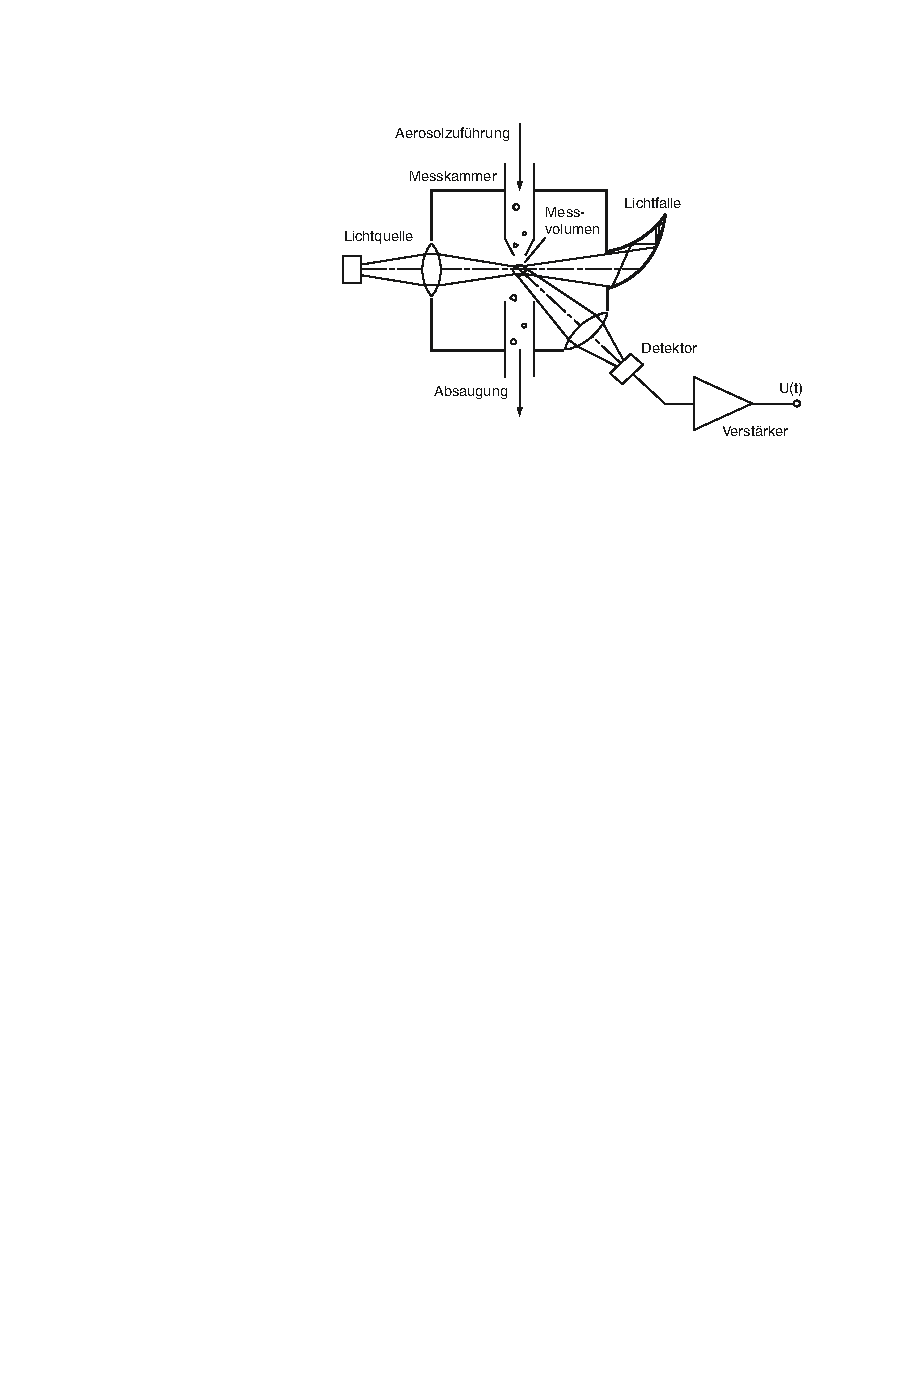
\includegraphics[width=.9\linewidth]{gfx/requirements/optischer_messer.pdf}} \quad
	\caption[Funktionsprinzip eines optischen Partikelz\"{a}hlers (Quelle: \cite{reinraum}, S.75)]
	{Funktionsprinzip eines optischen Partikelz\"{a}hlers (Quelle: \cite{reinraum}, S.75)}
	\label{fig:optischer_messer}
\end{figure}

\begin{figure}[H]
	\myfloatalign
	{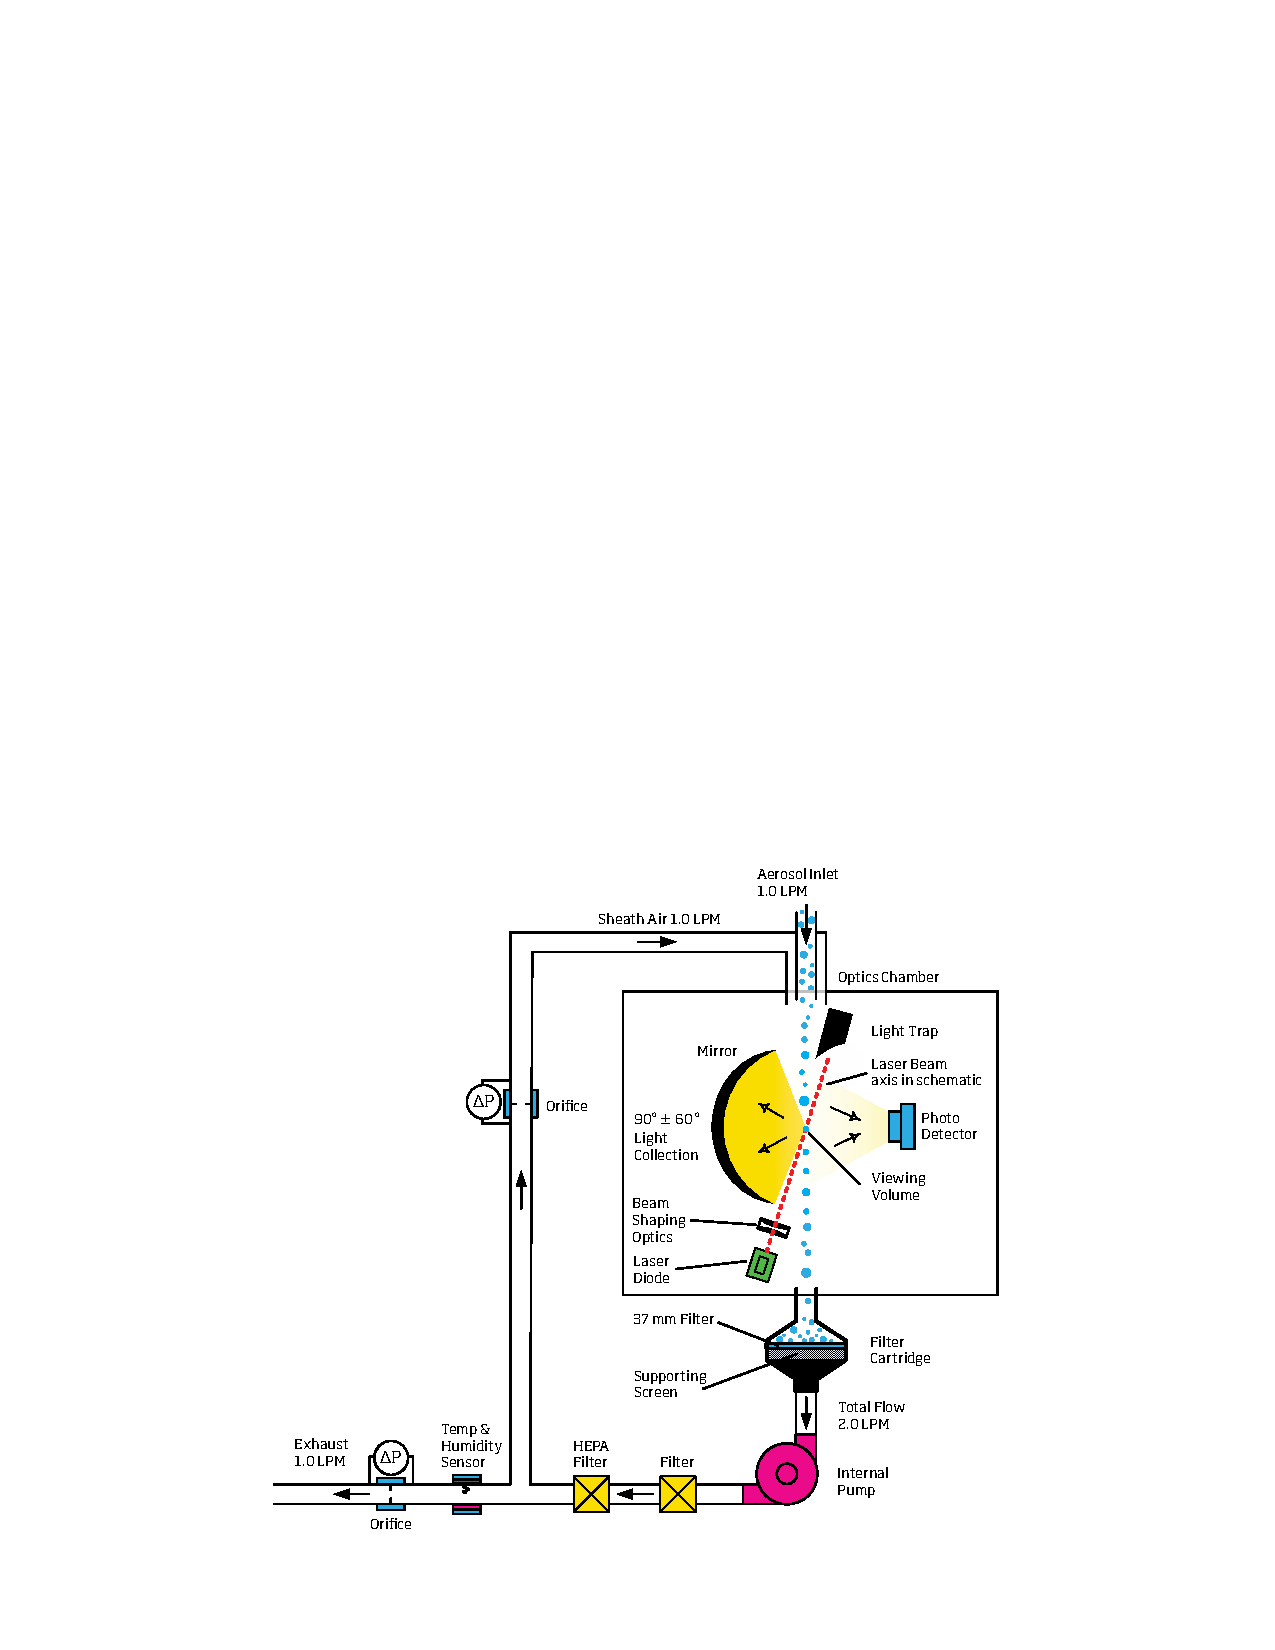
\includegraphics[width=.9\linewidth]{gfx/requirements/ops_3330.pdf}} \quad
	\caption[Lasermessung beim OPS 3330 (Quelle: \cite{ops_3330}, S.2)]
	{Lasermessung beim OPS 3330 (Quelle: \cite{ops_3330}, S.2)}
	\label{fig:laser_messer}
\end{figure}

\begin{figure}[H]
	\myfloatalign
	{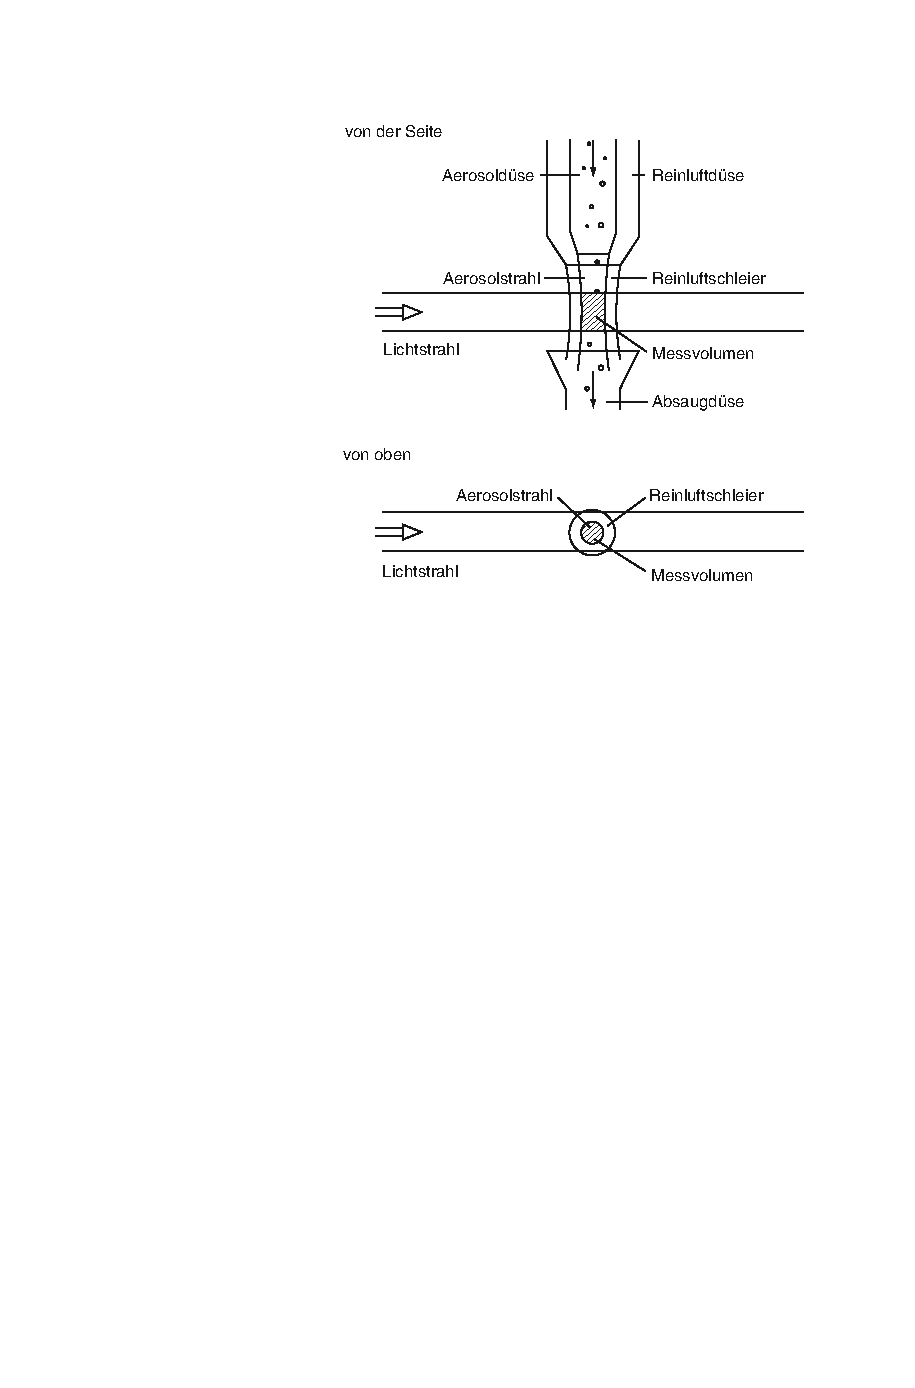
\includegraphics[width=.9\linewidth]{gfx/requirements/aerodynamisch_fokus.pdf}} \quad
	\caption[Messvolumentrennung durch aerodynamische Fokussierung (Quelle: \cite{reinraum}, S.76)]
	{Messvolumentrennung durch aerodynamische Fokussierung (Quelle: \cite{reinraum}, S.76)}
	\label{fig:aerodynamisch_trennung}
\end{figure}

\begin{figure}[H]
	\myfloatalign
	{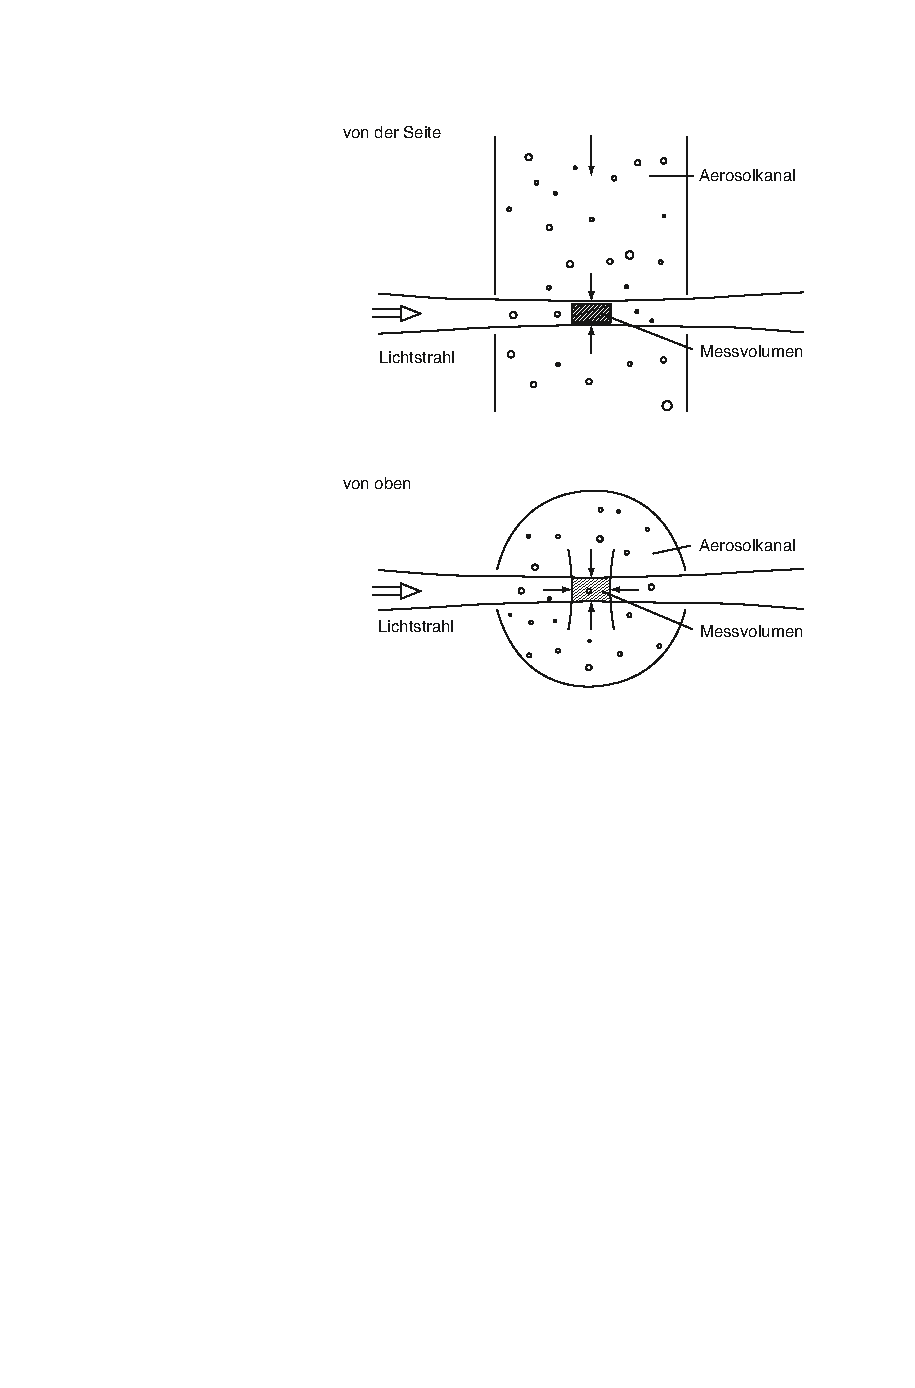
\includegraphics[width=.9\linewidth]{gfx/requirements/blenden_fokus.pdf}} \quad
	\caption[Messvolumentrennung mit Hilfe von Blenden (Quelle: \cite{reinraum}, S.77)]
	{Messvolumentrennung mit Hilfe von Blenden (Quelle: \cite{reinraum}, S.77)}
	\label{fig:optisch_trennung}
\end{figure}

Elektrische Pertikelz\"{a}hler wie der FMPS 3091 hingegen ben\"{o}tigen keine speziellen Techniken, um Partikel einzeln zu erfassen. Beim FMPS 3091 werden die Partikel positiv aufgeladen und dann mit einem reinen Luftstrom in das Messvolumen gef\"{u}hrt, in welchem sich eine Elektrode befindet und ein elektrisches Feld erzeugt. Elektrometer, welche um die Eletrode angebracht sind und verschieden emfindlich sind, messen die geladenen Partikel (Abbildung \ref{elektrisch_messer}).

\begin{figure}[H]
	\myfloatalign
	{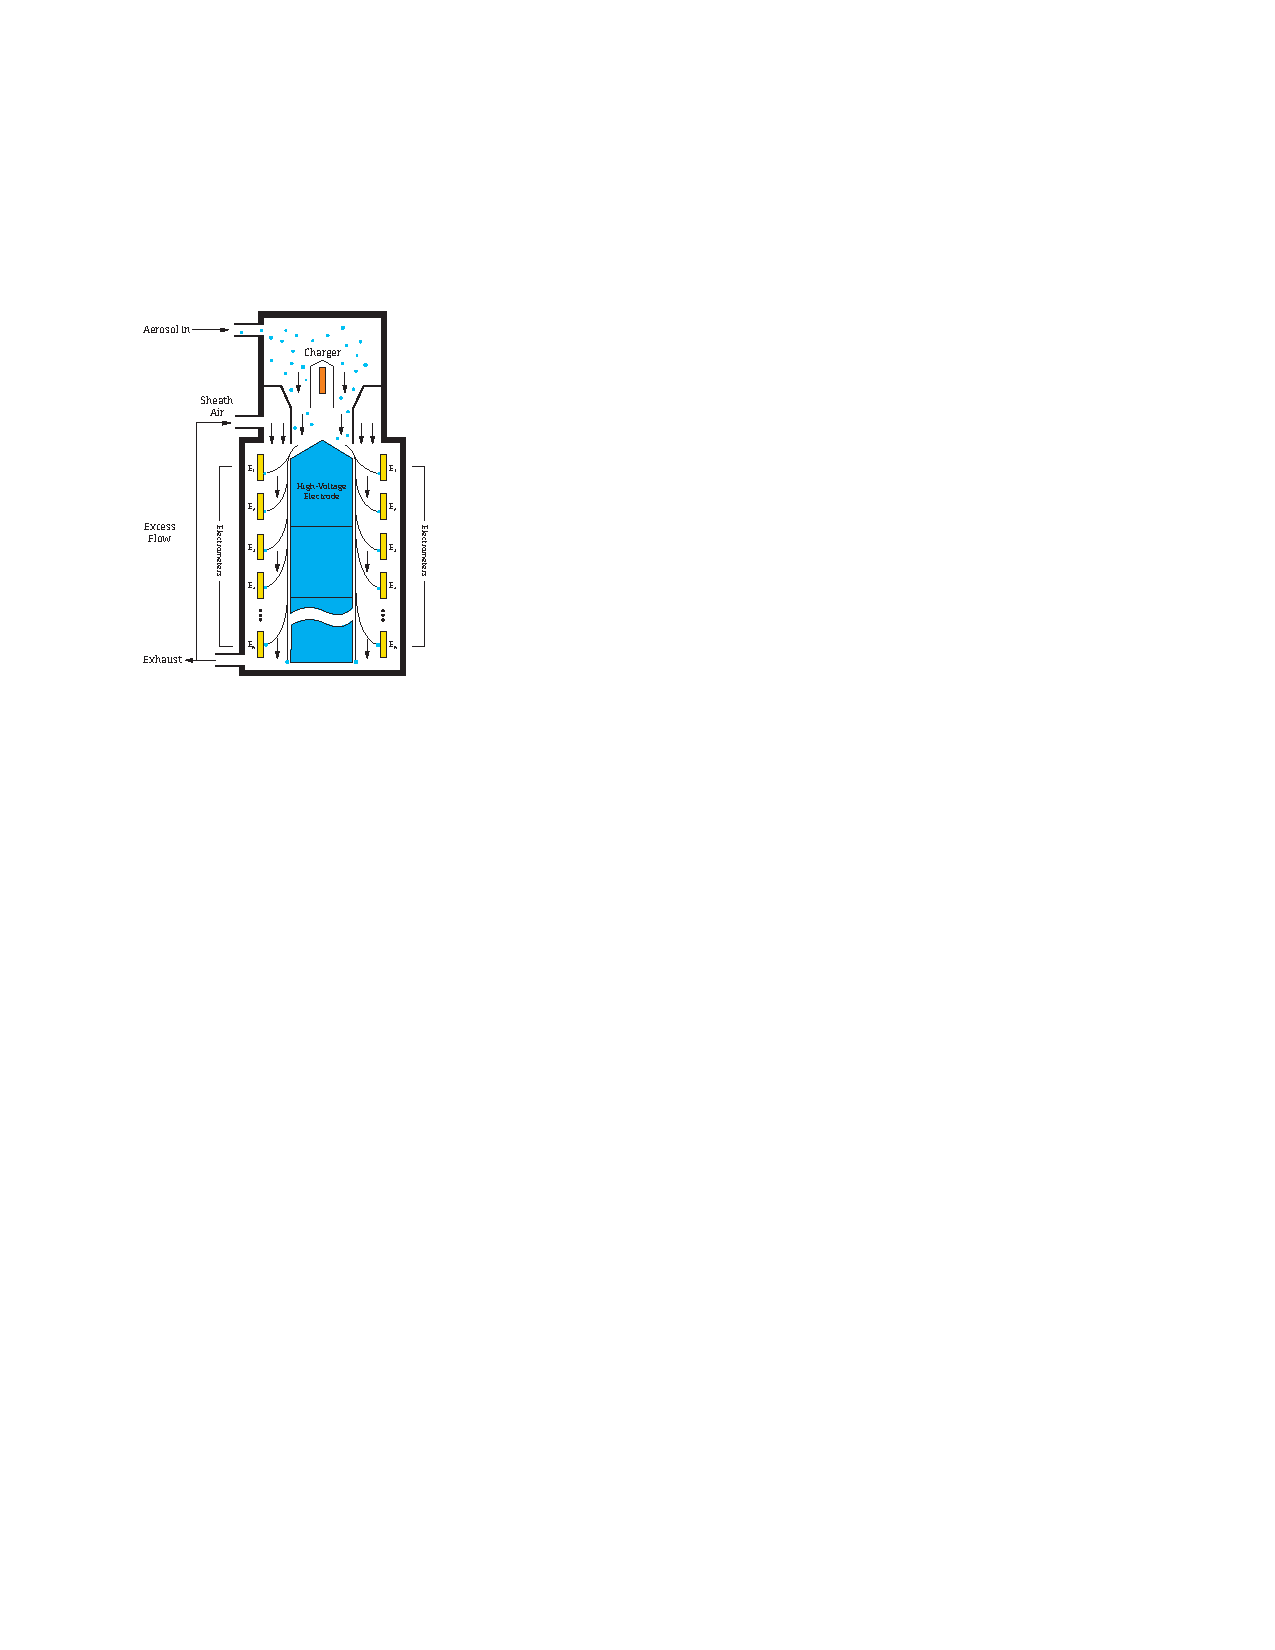
\includegraphics[width=.9\linewidth]{gfx/requirements/fmps_3091.pdf}} \quad
	\caption[Elektrische Messung beim FMPS 3091 (Quelle: \cite{fmps_3091}, S.6)]
	{Elektrische Messung beim FMPS 3091 (Quelle: \cite{fmps_3091}, S.6)}
	\label{fig:elektrisch_messer}
\end{figure}

Ein wesentlicher Leistungsunterschied zwischen dem FMPS 3091 und OPS 3330 ist das Volumen des Aerosol-Luftgemisches, welches von beiden im Verh\"{a}ltnis 1:4 angesaugt wird. Der OPS arbeitet mit $5 L/min$, w\"{a}rend der FMPS mit $50 L/min$ arbeitet. Ein Teil des Luftgemisches wird dabei vom Ger\"{a}t gefiltert und dazu genutzt, den Aerosolstrom zum Messvolumen zu f\"{u}hren.   

\subsection{Aerosolquelle}
Die Aerosolquelle liefert mit dem Aerosol, den entscheidenden Faktor zum Partikelsprung. Aus den Begrenzungen der Messger\"{a}te sowie allgemeiner Richtlinien zur Aerosolgenerierung ergeben sich folgende Anforderungen.

\begin{itemize}
\item \textbf{Einhaltung eines vorgegebenen Druckbereiches(1)}\\
Die internen Pumpen, welche den Volumenstrom der Messger\"{a}te regulieren, arbeiten nur in einem bestimmten Druckbereich korrekt(Q). Dieser Druckbereich begrenzt wiederum den Aerosoldruck, welcher am Messger\"{a}t-Einlass herrschen darf. Es ist darauf zu achten, dass die Aerosolquelle diesen Druckbereich einh\"{a}lt(Q). 
Auch das Design der Aerosolleitungen und der Schaltvorrichtung beeinflussen den Druck am Messger\"{a}t-Einlass. 
Quellen: \cite{fmps_3091}, \cite{ops_3330}, \cite{aps_3321}, \cite{ucpc_3776}, \cite{tsl_skript}

\item \textbf{Regulationszeit des Aerosolquelle(2)}\\
Die Einstellzeit einer Leistungskenngr\"{o}{\ss}e beschreibt das dynamische Verhalten der Aerosolquelle bez\"{u}glich dieser Gr\"{o}{\ss}e bei sprungf\"{o}rmigen \"{A}nderungen eines Einstellparameters. Dabei ist vor allem die Einstellzeit der Partikelanzahlkonzentration f\"{u}r den Versuchsaufbau interessant(Q). 
Quellen: \cite{vdi3491}

\item \textbf{Auswahl eines Tr\"{a}gergases(3)}\\
Das Tr\"{a}gergas der Aerosole hat einen gro{\ss}en Einfluss auf das Messverhalten der Messger\"{a}te.  F\"{u}r den Versuchsaufbau kommt vor allem gereinigte Luft als Tr\"{a}gergas in Frage, da diese auch bei der Messung der Bremspartikel als Tr\"{a}gergas fungiert und die ausgew\"{a}hlten Messger\"{a}te mit Luft oder Inertgas (UCPC) arbeiten(Q). 
Quellen: \cite{fmps_3091}, \cite{ops_3330}, \cite{aps_3321}, \cite{ucpc_3776}

\item \textbf{Bereitstellen eines ausreichenden Volumenstroms(4)}\\
Die Messger\"{a}te arbeiten mit einem fest vorgegebenen Volumenstrom des Tr\"{a}gergases.  Es muss gew\"{a}hrleistet sein, dass die Aerosolquelle einen entsprechenden Strom bereitstellen kann. Sollte der Volumenstrom den Anforderungen nicht entsprechen, generieren die Messger\"{a}te eine Fehlermeldung und liefern keine Messwerte mehr(Q). 
Quellen: \cite{fmps_3091}, \cite{ops_3330}, \cite{aps_3321}, \cite{ucpc_3776}

\item \textbf{Einhalten von Temperaturgrenzen(5)}\\ 
Die Tr\"{a}gergastemperatur kann je nach Aerosolquelle verschiedene Werte annehmen. Da die Temperatur des Aerosols den Messprozess und die Eigenschaften des Aerosolstromes beeinflusst, geben die Messger\"{a}tehersteller feste Temperaturgrenzen vor zwischen welchen sich diese Temperatur bewegen darf(Q). 
Quellen: \cite{fmps_3091}, \cite{ops_3330}, \cite{aps_3321}, \cite{ucpc_3776}
\end{itemize}

\subsection{Aerosol}
Folgende Anforderung an das Aerosol ergeben sich aus den Arbeitsbereichsbegrenzungen der Messger\"{a}te und aus der statistischen Verwertbarkeit der Messwerte zur Berechnung des zeitlichen Verhaltens der Messger\"{a}te.

\begin{itemize}
\item \textbf{Einhalten der Partikelanzahlkonzentration(6)}\\
Eine zu hohe Partikelanzahlkonzentration f\"{u}hrt zu einer H\"{a}ufung von falschen Messergebnissen zum Beispiel durch Koinzidenz bei optischen Sensoren. Messergebnisse bei einer zu niedrigen Partikelanzahlkonzentration k\"{o}nnen bei Messger\"{a}ten, welche mit elektrischen Feldern arbeiten, in dem herrschenden, systematischen Grundrauschen untergehen. Somit muss f\"{u}r verwertbare Ergebnisse die Partikelanzahlkonzentration des Aerosols mit dem benutzten Messger\"{a}t abgeglichen werden(Q).
Quellen: \cite{fmps_3091}, \cite{ops_3330}, \cite{aps_3321}, \cite{ucpc_3776}

\item \textbf{Wahl des Partikelmaterial(7)} 
Partikelmaterialien k\"{o}nnen Gesundheits- oder Umweltgef\"{a}hrdend sein oder aufgrund von ihren Eigenschaften f\"{u}r bestimmte Messverfahren nicht geeignet sein. Deswegen ist es wichtig das benutzte Partikelmaterial zu kennen. Da die hier benutzten Messger\"{a}te vor allem f\"{u}r die Feinstaubmessung benutzt werden, bieten sich zum Beispiel feste Materialien f\"{u}r die Aerosole an(Q).
Quellen: \cite{vdi3491}

\item \textbf{Wahl der Partikelgr\"{o}{\ss}e(8)}\\ 
Zu kleine Partikel k\"{o}nnen von den Messsystemen der Partikelz\"{a}hler nicht erfasst werden, w\"{a}hrend zu gro{\ss}e Partikel durch Verstopfen der Filter die Funktion beeintr\"{a}chtigen k\"{o}nnen. Manche Hersteller geben an, dass zu gro{\ss}e Partikel zwar gez\"{a}hlt werden, aber nicht mehr in die Gr\"{o}{\ss}enverteilung mit eingehen. Trotzdem sollte zur Sicherheit ein Zyklonabscheider dem System zugeschaltet werden, wenn nicht garantiert werden kann, dass nicht zu viele zu gro{\ss}e Partikel im Aerosol sind(Q).
Quellen: \cite{fmps_3091}, \cite{ops_3330}, \cite{aps_3321}, \cite{ucpc_3776}
\end{itemize}

\subsection{Schaltvorrichtung}
Die Schaltvorrichtung ist das entscheidende Bauteil beim Erzeugen der Sprungfunktion. Dabei sind ein schneller Schaltprozess aber auch ein str\"{o}mungsg\"{u}nstiges Design f\"{u}r die G\"{u}te der Schaltvorrichtung die ausschlaggebenden Kriterien. Auch das Material kann hierbei eine Rolle spielen. Folgende Anforderungen lassen sich definieren.

\begin{itemize}
\item \textbf{Erreichen einer kurzen Schaltzeit(9)}\\
Die Zeit, die die Vorrichtung ben\"{o}tigt um von einem Schaltzustand in den anderen zu wechseln, sollte so kurz wie m\"{o}glich sein. Diese Schaltzeit tr\"{a}gt zur Totzeit des Versuchsaufbaus bei. 
	
\item \textbf{Erreichen eines Str\"{o}mungsbeg\"{u}nstigenden Schaltvorgangs(10)}\\ 
Hochwinklige Umlenkungen und abrupte Querschnitts\"{a}nderungen k\"{o}nnen zu Partikel- und Druckverlusten f\"{u}hren. Somit k\"{o}nnen sie die G\"{u}te der Partikelfront beeinflussen und sollten deswegen vermieden werden. Außerdem kann es bei ung\"{u}nstigem Design der Schaltvorrichtung zu Turbulenzen in ihrem Inneren kommen, was die Berechenbarkeit der Totzeit des Aufbaus erheblich erschwert. Die vorhergehenden \"{U}berlegungen gelten auch f\"{u}r die Auslegung der Aerosolleitung, (Q).
%TODO (Hiwis vom Windkanal) 
\end{itemize}

\subsection{Aerosolleitungen}
Auch bei der Leitung des Aerosols, ist auf eine str\"{o}mungsg\"{u}nstige Auslegung zu achten. Dies betrifft die Ausma{\ss}e, das Material, den Zustand der Innenfl\"{a}chen und die r\"{a}umliche F\"{u}hrung der einzelnen Verbindungen. Die folgenden Anforderungen k\"{o}nnen also auch als Designkriterien angesehen werden.

\begin{itemize}
\item \textbf{Str\"{o}mungsweg des Versuchaufbaus(11)}\\ 
Der Weg zwischen der Umschaltvorrichtung und dem Messger\"{a}teeinlass f\"{u}hrt bei gegebenen Volumenstr\"{o}men, abh\"{a}ngig von dem benutzten Messger\"{a}t, zu einer Verz\"{o}gerungszeit, die sich in der Totzeit des Versuchsaufbaus niederschl\"{a}gt. Da das Str\"{o}mungsverhalten in den Verbindungen nur unter Annahme von Vereinfachungen zutrifft, gilt: Umso l\"{a}nger der Weg ist, umso gr\"{o}{\ss}er ist der Rechenfehler bei der Berechnung der Totzeit. Au{\ss}erdem f\"{u}hren Druck- und Partikelverluste auf diesem Weg zu einer Verzerrung der Partikelfront. (Q)
Quellen: \cite{vdi3491}

\item \textbf{Erreichen eines laminaren Stroms(12)}\\ 
Da eine turbulente Str\"{o}mung zu einem analytisch kaum berechenbaren Verhalten der Str\"{o}mung f\"{u}hrt, ist der Versuchsaufbau so zu gestalten, dass sich die Str\"{o}mung m\"{o}glichst \"{u}berall laminar verh\"{a}lt (Q). Vor allem am Messger\"{a}te- Einlass, wo es zu einem Querschnitts\"{u}bergang kommen kann, sollten entsprechend gestaltete Adapter daf\"{u}r Sorge tragen.
Quellen: \cite{vdi3491}

\item\textbf{Flexible Schnittstelle zwischen Messger\"{a}t und Versuchsaufbau(13)}\\ 
Die Messger\"{a}te besitzen einen Aerosoleinlass in Form eines R\"{o}hrchens mit unterschiedlichen Durchmessern, welches in die Umgebung ragt(Q). Je nach Versuchsaufbau k\"{o}nnen Adapter von N\"{o}ten sein, um eine direkte Verbindung zwischen Schaltvorrichtung und Messger\"{a}t zu gew\"{a}hrleisten. Bei der Gestaltung dieser Adapter muss ein Kompromiss zwischen Anforderung 12 und 13 eingegangen werden.
Quellen: \cite{fmps_3091}, \cite{ops_3330}, \cite{aps_3321}, \cite{ucpc_3776}
\end{itemize}

\subsection{Versuchsaufbau}
\begin{itemize}
\item \textbf{Optimale Pr\"{u}fzeit(14)}\\ 
Die minimale Versuchszeit ist wichtig in der Versuchsplanung, da durch die Messaufl\"{o}sung der Messger\"{a}te von einer Sekunde, die Anzahl der Messwerte je nach Versuchsaufbau begrenzt ist. Nun kann eine Versuchsdurchf\"{u}hrung aus mehreren Abl\"{a}ufen (abwechselnd: gereinigte Luft (zb. 5 s) -- Aerosol(zb. 30s)) und die Abl\"{a}ufe wiederum aus mehreren Messungen (der Partikelanzahl) bestehen. Je nach Varianz der Partikelanzahl, sind eine bestimmte Anzahl von Messungen und Messabl\"{a}ufen von N\"{o}ten um ein valides Ergebnis f\"{u}r die Zeitkonstante zu erhalten. So sollte der Aufbau ca. 100 Abl\"{a}ufe mit je 30 Partikelanzahlmessungen (+ 5 Sekunden gereinigte Luft pro Ablauf) mit reproduzierbaren Ergebnissen liefern k\"{o}nnen.

\item \textbf{Annehmbare Kosten(15)}\\
Aus wirtschaftlicher Sicht, sind die Kosten ein ausschlaggebender Faktor für die G\"{u}te des Aufbaus. Sie setzen sich aus den Materialkosten selbstgestalteter und eventuell selbstgebauter Teile, den Kosten für Zukaufteile, wie Filter, Verdichter, Aerosolgeneratoren etc. und den Kosten f\"{u}r Ressourcen, wie Strom, Aerosol etc., zusammen. Die maximalen Kosten d\"{u}rfen die vorgegebenen Mittel des Fachgebietes nicht \"{u}berschreiten. 

\item \textbf{Flexibilit\"{a}t f\"{u}r verschiedene Ger\"{a}te(16)}\\
Ziel des Aufbaus ist die Evaluation der Dynamik von Messger\"{a}ten, welche f\"{u}r Messungen von Bremspartikeln am Schwungmassenpr\"{u}fstand ben\"{o}tigt werden. Von den f\"{u}nf f\"{u}r diesen Zweck ausgesuchten Messger\"{a}ten, wurden vor allem der FMPS 3091 und der OPS 3330 f\"{u}r geeignet befunden. Nun sollen die, durch den hier konstruierten Versuchsaufbau, ermittelten Werte zumindest f\"{u}r diese beiden Ger\"{a}te ein valides Ergebnis darstellen. Jedes weitere Messger\"{a}t, das durch den Aufbau erfolgreich getestet werden kann, erh\"{o}ht dessen wirtschaftlichen und wissenschaftlichen Wert.
\end{itemize}